\chapter{Preparation}

\section{Theory}

\subsection{Slab Waveguide}
\subsubsection{Calculation of Modes}
\subsubsection{Field Distribution and Dispersion Diagramm}


\subsection{Strip Waveguide}



\section{Questions}

\subsection{Slab and Strip waveguide?}
\label{q1}
<<<<<<< HEAD
% A waveguide usualy consists of a core material with a destinct refractive index surrounded by a cladding with another refractive index. For planar waveguides the lower layer is usualy called substrate. For guiding modes in the waveguide the refractive indices of the core has to be higher than the refractive indices of the cladding and substrate.
A slab waveguide consists of three lateral infinitly spread layers  with different refractive indices (cf. figure \ref{fig:}). In planar waveguide structures the upper layer is usualy called cladding, the middle layer core and the lower layer substrate. The strip waveguide also consists of these layers but the core is not infinitely spread (cf. figure \ref{fig:}). It rather has a destinct width in one direction. Thus the field is confined in two dimensions.

For guiding modes the refractive index in the core has to be higher than the refractive index in the cladding and the substrate. Common materials for a such waveguides are SiO$_2$ (n $\approx 1.47$) as Substrate, Si (n $\approx 3.5$) as core and some Polymere (n $\approx 1.5$) as cladding.
=======
A slab waveguide is a structure of several layers of different materials. The structures are extended infinitely. The middle layer has the highest refractive index. Here the electric field is confined and the wave is guided.
Figure \ref{fig:slab} shows the schematic layout of a slab waveguide and the index profile of this structure. 
As materials and therefore refractive indices for the cladding and the Substrate SiO$_2$ with $n_2 = 1.44$ is selected. For the core region the refractive index of Silicon with $n_1 = 3.48$ is selected.

\begin{figure}%
\centering
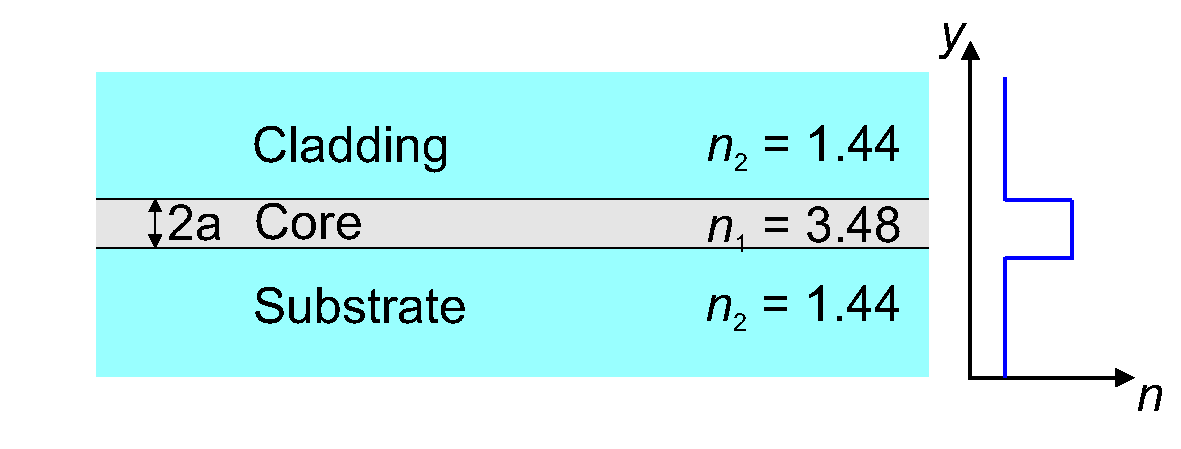
\includegraphics[width=.7\columnwidth]{Grafiken/swg.pdf}%
\caption{schematic layout of a slab waveguide}%
\label{fig:slab}%
\end{figure}

In contrast there is the strip waveguide. Here a strip of high-index material is placed on a lower index substrate. On top sometimes is a polymer or just air. Figure \ref{fig:strip} shows the schematic layout of a strip waveguide and the index profile at the marked position $x = 0$.

\begin{figure}%
\centering
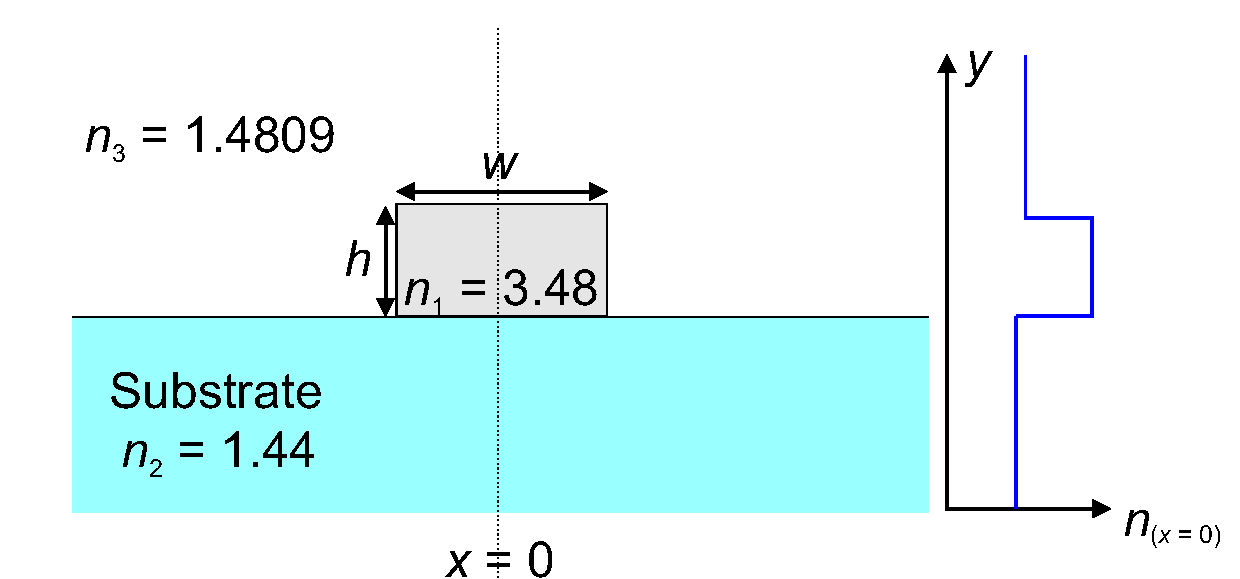
\includegraphics[width=.7\columnwidth]{Grafiken/strip.pdf}%
\caption{schematic layout of a strip waveguide}%
\label{fig:strip}%
\end{figure}
>>>>>>> a2e6dd7e6b29e9572d504606d089c8c1a2da7d39
\comseb{hmm, die versionen sind beide gut, wir m�ssen uns f�r eine entscheiden. bei dir vermiss ich die bezeichnungen cladding und substrate}
\subsection{Different performance between TE and TM @ boundary}
There are different kinds of polarizations. The TE-polarized wave has the boundary conditions:\\
$\vec{\mathrm{E}}_i ~\bot~$plane of incidence\\
and\\
$\vec{\mathrm{H}}_i ~||~$ plane of incidence.\\

For the TM-polarized wave the following boundary conditions are given:\\
$\vec{\mathrm{H}}_i ~\bot~$plane of incidence\\
and\\
$\vec{\mathrm{E}}_i ~||~$ plane of incidence.\\
Any other polarization states can be interpreted as a superposition of a TE and a TM wave.

The TE-modes have always a larger propagation constant than the TM-modes. TE-modes are more confined to the high-index core region than the TM modes.\footnote[1]{Christian Koos, Optical Waveguides and Fibres, Lecture Notes}


\subsection{Single Mode strip waveguide}

\begin{figure}%
\centering
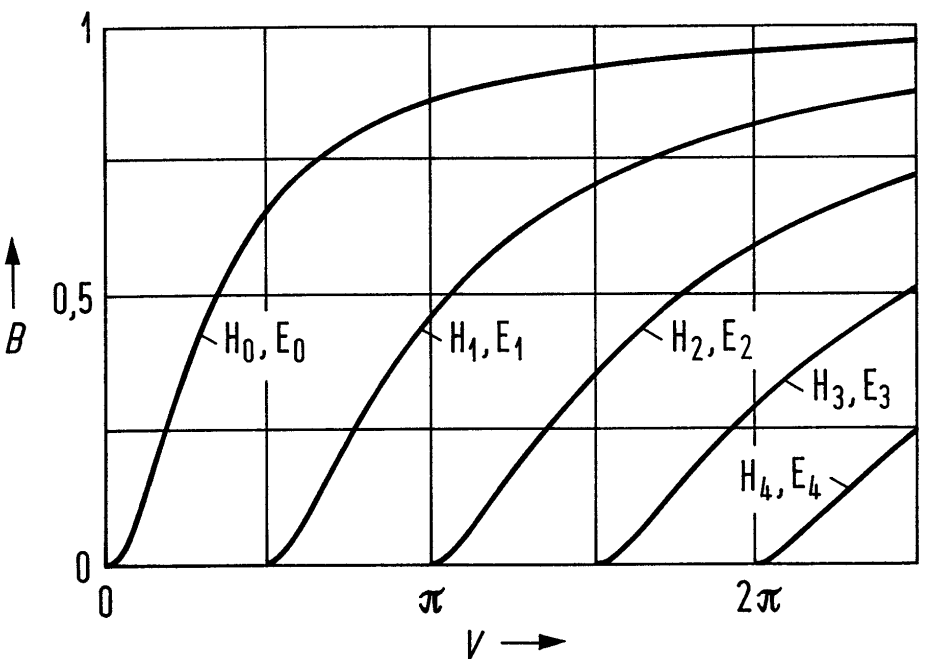
\includegraphics[width=.5\columnwidth]{Grafiken/SingleMode.png}%
\caption{Normalized propagation $B$ over normalized frequency $V$ for a low index contrast.}%
\label{fig:singlemoded}%
\end{figure}
To achieve a single mode strip waveguide the normalized frequency $V$ needs to be smaller than $\pi/2$. This can be explained by looking at the dispersion relation in Figure \ref{fig:singlemoded}\footnote[1]{Wolfgang Freude, Optische Wellenleiter und Sender, Lecture Notes}. For a normalized frequency $V$ a modes with the corresponding normalized wavenumber $B$ are guided. The normalized frequency calculates as:
\begin{equation}
V=ak_0\sqrt{n_1^2-n_2^2}
\label{eq:norm_freq}
\end{equation}
with $2a$ is the thickness of the core, $n_1$ is the refractive index of the core, $n_2$ is the refractive index of the cladding and $k_0 = 2\pi/\lambda$ is the wavenumber. Thus the parameters which determine the number of modes in a waveguide are the thickness of the core layer $2a$, the wavelength $\lambda$ and the refractive indices of the waveguide materials. For $V < \pi/2$ only the fundamental mode is guided. Note that there are still two polarizations H$_0$ and E$_0$.

\todo{wir ham nen asymetrischen waveguide angenommen, das bild is f�r symetrisch}
For the in \ref{q1} values assumed for $n_1$ and $n_2$ this leads to a core-thickness of
\begin{equation}
2a>\frac{\pi}{k_0\sqrt{n_1^2-n_2^2}}=\frac{\lambda_0}{2\sqrt{n_1^2-n_2^2}}=2.45~\cdot~10^{-7}~\mathrm{m}
\label{eq:}
\end{equation}
for $\lambda_0$ = 1550~nm, $n_1 = 3.48$ and $n_2 = 1.44$. 
That means when using a Silicon core with a hight of 245~nm the slab waveguide is single moded f�r $\lambda_0 < 1.55~\upmu$m.
